\documentclass[11pt]{article}
\usepackage[
  paperheight=2.125in, 
  paperwidth=5.5in,
  margin=.3in
]{geometry}
\usepackage{tikz,graphicx}
\usetikzlibrary{shadings,decorations.pathmorphing}

\tikzstyle{vector}=[
  ->,
  red,
  thick
]


\begin{document}
\pagestyle{empty}

\paragraph{Ex \#1} 

You hike 20 meters east and then 40 meters north.  What is your displacement (magnitude and direction)?

\begin{center}
  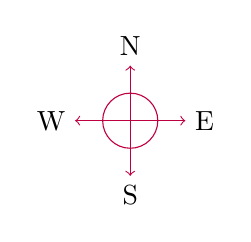
\begin{tikzpicture}[scale=0.7,draw=purple]
    \draw[<->] 
      (1,0) node[right] {E} 
      -- (-1,0) node[left] {W};
    \draw[<->]
      (0,1) node[above] {N} 
      -- (0,-1) node[below] {S};
    \draw (0,0) circle (0.5);

  \end{tikzpicture}
\end{center}

\pagebreak

\paragraph{Ex \#2} 

You row east across a river at a speed of 7 m/s.  The river flows north at a speed of 3 m/s.  From the perspective of someone standing on the shore, what is your velocity (magnitude and direction)?


\begin{center}
  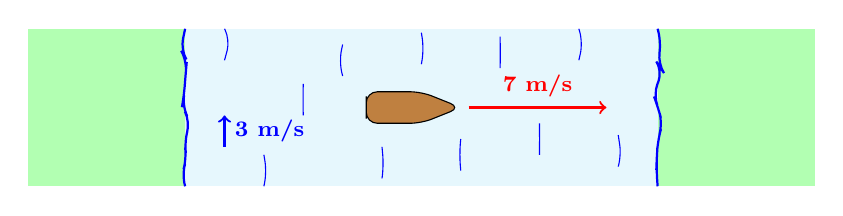
\begin{tikzpicture}
    \begin{scope}
      \tikzstyle{riverbank}=[
        blue, thick, 
        decorate, 
        decoration={
          random steps,
          segment length=2mm,
          amplitude=2pt
        },
        rounded corners
      ]
      \tikzstyle{water}=[
        blue, thin, 
        decorate, 
        decoration={
          random steps,
          segment length=2mm,
          amplitude=2pt
        },
        rounded corners
      ]
      \fill[green!30] (-1,-1) rectangle ++ (-2,2);
      \fill[green!30] (5,-1) rectangle ++ (2,2);
      \fill[cyan!10] (-1,-1) rectangle ++ (6,2);
      \draw[riverbank]
        (-1,-1) -- ++(0,2);
      \draw[riverbank] (5,-1) -- ++(0,2);
      \draw[vector,blue] (-0.5,-0.5)
         -- ++(0,0.4) node[midway,right] 
         {\footnotesize \bf 3 m/s};
      \draw[water] (-.5,.6) -- ++(0,0.4);
      \draw[water] (0,-1) -- ++(0,0.4);
      \draw[water] (0.5,-0.1) -- ++(0,0.4);
      \draw[water] (1,0.4) -- ++(0,0.4);
      \draw[water] (1.5,-.9) -- ++(0,0.4);
      \draw[water] (2,.55) -- ++(0,0.4);
      \draw[water] (2.5,-0.8) -- ++(0,0.4);
      \draw[water] (3,0.5) -- ++(0,0.4);
      \draw[water] (3.5,-.6) -- ++(0,0.4);
      \draw[water] (4,.6) -- ++(0,0.4);
      \draw[water] (4.5,-0.75) -- ++(0,0.4);
    \end{scope}
    \begin{scope}[rounded corners]
      \draw[fill=brown] (1.3,0)
        -- ++(0,.2)
        -- ++(.7,0)
        -- ++(.5,-.2) coordinate (boat front)
        -- ++(-.5,-.2)
        -- ++(-.7,0)
        -- cycle;
    \end{scope}
    \draw[vector] 
      (boat front) ++(0.1,0) -- ++(1.75,0)
      node[midway, above] 
        {\footnotesize \bf 7 m/s};
  \end{tikzpicture}
\end{center}

\pagebreak

\paragraph{Ex \#3} 

A ball is thrown with an initial resultant velocity of 12.5 m/s at angle 53$^\circ$ above horizontal.  Calculate the $x$- and $y$- components of the ball's initial velocity.

\begin{center}
  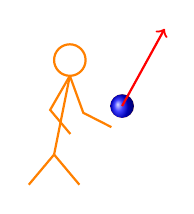
\begin{tikzpicture}
    \begin{scope}[thick, orange]
      \draw (0,1.2) circle (0.2);
      \coordinate (waiste) at (-.2,0);
      \coordinate (neck) at (0,1);
      \draw (waiste) -- (neck);
      \draw (waiste) -- ++(230:0.5);
      \draw (waiste) -- ++(310:0.5);
      \draw (neck) -- ++(-70:0.5) 
        -- ++(-27:0.4) coordinate (throwing hand);
      \draw (neck) -- ++(-120:0.5) 
        -- ++(-50:0.4);
      \fill[shading=ball] (throwing hand) ++ (63:0.3) coordinate(ball) circle (0.15);
      \draw[vector] (ball) -- (53:2);
    \end{scope}
  \end{tikzpicture}
\end{center}

\pagebreak

\paragraph{Ex \#4} 

An airplane comes in for a landing at a speed of 67 m/s.  Its angle is 15 degrees below horizontal.  Calculate the $x$- and $y$- components of the airplane's velocity.

\begin{center}
  \begin{tikzpicture}
    \node at (0,0) 
      {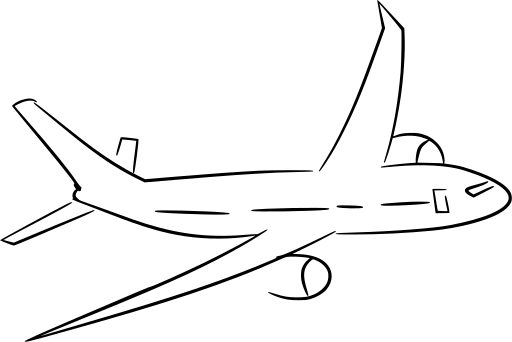
\includegraphics[angle=-15,origin=c,width=1.5cm]{airplane.png}};
    \draw[vector] (.6,-.2) coordinate (a)
      -- ++(-15:2.05) 
      node[midway, below, rotate=-14] 
      {\footnotesize 67 m/s};
    \draw[dashed, thin] (a) -- ++(3,0);
    \draw (-3,-1.1) -- ++(9,0);
    \node at (2.1,-.4) {\footnotesize $15^\circ$};
  \end{tikzpicture}
\end{center}


\end{document}